This chapter will go into the results of the simulation and the validation of the success of the chosen approach.

Functions ($\mathbb{R}^2 \mapsto \mathbb{R}$):

\begin{enumerate}
	\item $f(n, t) = w_n n + w_tt$
	\item $g(n, t) = \frac{w_n n^2}{2} + \frac{w_t t^2}{2}$
	\item $h(n, t) = (n + t)(n + c)$
	\item $i(n, t) = n$
\end{enumerate}

\begin{figure}
\centering	
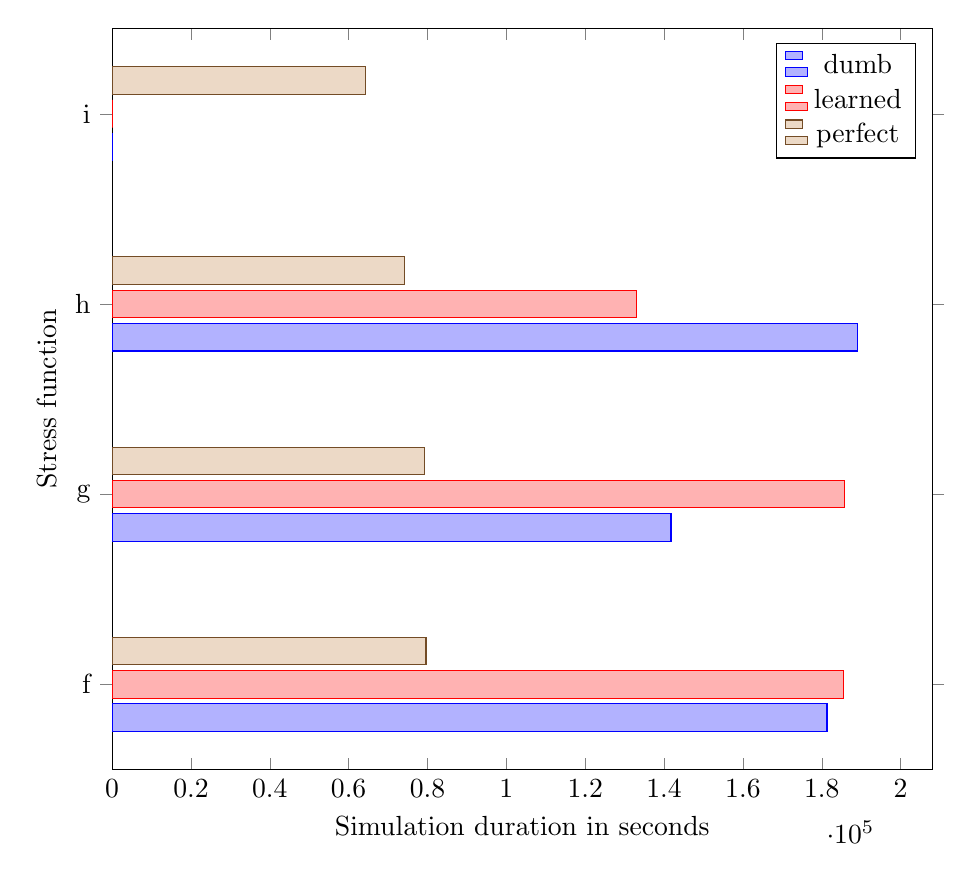
\begin{tikzpicture}
\begin{axis}[
	xbar,
	xmin=0,
	width=12cm,
	height=11cm,
	enlarge y limits=0.15,
	xlabel={Simulation duration in seconds},
	ylabel={Stress function},
	symbolic y coords={f,g,h,i},
	ytick=data,
	nodes near coords align={horizontal},
]
\addplot coordinates {(0,i) (189149,h) (141760,g) (181329,f)};
\addplot coordinates {(0,i) (132996,h) (185709,g) (185400,f)};
\addplot coordinates {(64249,i) (74127,h) (79132,g) (79625,f)};
\legend{dumb,learned,perfect}
\end{axis}
\end{tikzpicture}
\label{stress_based_results}
\caption{Simulation durations for the stress based signal controller.}
\end{figure}

\begin{figure}
	\centering	
	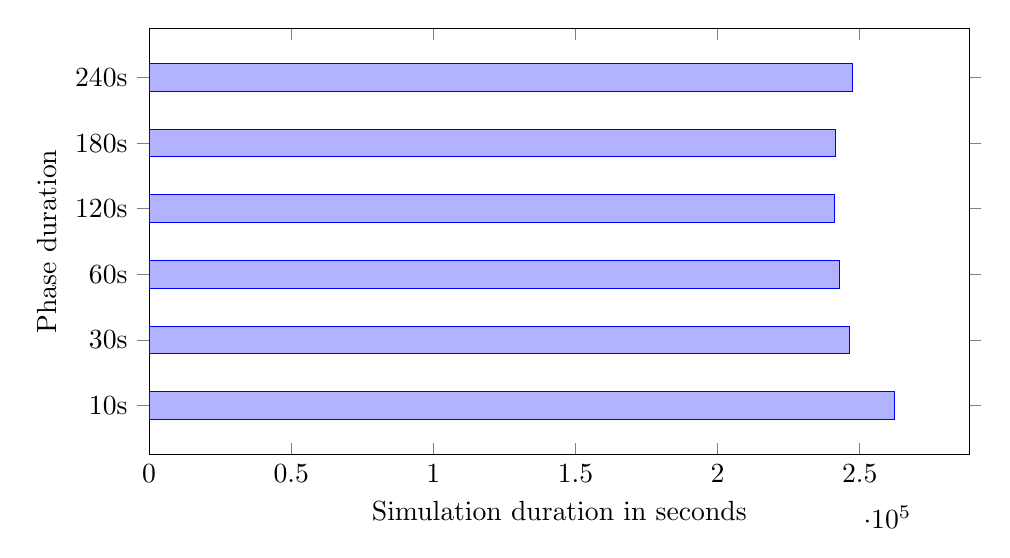
\begin{tikzpicture}
	\begin{axis}[
			xbar,
			xmin=0,
			width=12cm,
			height=7cm,
			enlarge y limits=0.15,
			xlabel={Simulation duration in seconds},
			ylabel={Phase duration},
			symbolic y coords={10s,30s,60s,120s,180s,240s},
			ytick=data,
			nodes near coords align={horizontal},
		]
		\addplot coordinates {(262385,10s) (246490,30s) (242953,60s) (240975,120s) (241523,180s) (247402,240s)};
		\end{axis}
	\end{tikzpicture}
	\label{cycle_based_results}
	\caption{Simulation durations for the fixed cycle signal controller.}
\end{figure}

\begin{figure}
	\centering
	\begin{tikzpicture}
	\begin{axis}[
		width=15cm,
		height=8cm,
		xmin=0,
		ymin=0,
		xlabel={Time in seconds},
		ylabel={Agents in the Network}
	]
	\addplot[mark=none,draw=red,thick] table [col sep=comma] {data/agents/cycle.csv};
	\addplot[mark=none,draw=blue,thick] table [col sep=comma] {data/agents/stress/dumb/sumnquadtlin.csv};
	\addplot[mark=none,draw=black,thick] table [col sep=comma] {data/agents/stress/dumb/sumnlintlin.csv};
	\addplot[mark=none,draw=purple,thick] table [col sep=comma] {data/agents/stress/dumb/sumnlinintegtlininteg.csv};
	\addplot[mark=none,draw=green,thick] table [col sep=comma] {data/agents/stress/dumb/nlin.csv};
	\legend{Cycle Controller, {h(n, t)}, {f(n, t)}, {g(n, t)}, {i(n, t)}}
	\end{axis}
	\end{tikzpicture}
	\label{agent_statistic_perfect}
	\caption{Agents living per time unit without previous learning.}
\end{figure}

\begin{figure}
	\centering
	\begin{tikzpicture}
	\begin{axis}[
		width=15cm,
		height=8cm,
		xmin=0,
		ymin=0,
		xlabel={Time in seconds},
		ylabel={Agents in the Network}
	]
	\addplot[mark=none,draw=red,thick] table [col sep=comma] {data/agents/cycle.csv};
	\addplot[mark=none,draw=blue,thick] table [col sep=comma] {data/agents/stress/learned/sumnquadtlin.csv};
	\addplot[mark=none,draw=black,thick] table [col sep=comma] {data/agents/stress/learned/sumnlintlin.csv};
	\addplot[mark=none,draw=purple,thick] table [col sep=comma] {data/agents/stress/learned/sumnlinintegtlininteg.csv};
	\addplot[mark=none,draw=green,thick] table [col sep=comma] {data/agents/stress/learned/nlin.csv};
	\legend{Cycle Controller, {h(n, t)}, {f(n, t)}, {g(n, t)}, {i(n, t)}}
	\end{axis}
	\end{tikzpicture}
	\label{agent_statistic_perfect}
	\caption{Agents living per time unit with previous learning.}
\end{figure}

\begin{figure}
	\centering
	\begin{tikzpicture}
	\begin{axis}[
		width=15cm,
		height=8cm,
		xmin=0,
		ymin=0,
		xlabel={Time in seconds},
		ylabel={Agents in the Network}
	]
	\addplot[mark=none,draw=red,thick] table [col sep=comma] {data/agents/cycle.csv};
	\addplot[mark=none,draw=blue,thick] table [col sep=comma] {data/agents/stress/perfect/sumnquadtlin.csv};
	\addplot[mark=none,draw=black,thick] table [col sep=comma] {data/agents/stress/perfect/sumnlintlin.csv};
	\addplot[mark=none,draw=purple,thick] table [col sep=comma] {data/agents/stress/perfect/sumnlinintegtlininteg.csv};
	\addplot[mark=none,draw=green,thick] table [col sep=comma] {data/agents/stress/perfect/nlin.csv};
	\legend{Cycle Controller, {h(n, t)}, {f(n, t)}, {g(n, t)}, {i(n, t)}}
	\end{axis}
	\end{tikzpicture}
	\label{agent_statistic_perfect}
	\caption{Agents living per time unit with perfect predictions.}
\end{figure}
